\documentclass[11pt,a4paper,oneside]{article}
\usepackage[utf8]{inputenc}
\usepackage{url}
\usepackage[pdftex]{graphicx}
\usepackage{float}
\usepackage{multicol}
\usepackage{color}
\usepackage{hyperref}
%\usepackage[T1]{fontenc}
%\usepackage{libertine}
%\renewcommand*\oldstylenums[1]{{\fontfamily{fxlj}\selectfont #1}}

\title{OSCELET\\
			\small{\url{https://github.com/mrkva/OSCELET}}}
\author{Jonáš Gruska \\
	\url{jonasgruska@gmail.com} \\
	Institute of Sonology \\
	The Hague, The Netherlands}
\date{\today}
\begin{document}
\maketitle

\section{Introduction}
OSCELET is ongoing project dealing with use of Kinect as control interface. It consists of application commuting Kinect data, particularly ``skeleton'' information via OSC to other software and development of various receiving clients in popular interactive audio languages (Max/MSP, Pure Data, Supercollider).

\section{OSCELET application}
The main OSCELET application is written in Processing. Its purpose is to grab data stream from Kinect device and analyze it in the same manner as the proprietary version of drivers on Microsoft Xbox does.

The code is based on the example by Max Rheiner, part of Simple OpenNI (Open Natural Interaction). Simple OpenNI is Processing port of OpenNI library, created by the organisation with the same name. Main purpose of OpenNI is to create a framework for dealing with natural interaction devices and applications.

My part was to implement OSC protocol using osc5 library and to optimize the code for the purposes of use. In current state, I have decided to use only upper-half of the body. I compiled the program for Mac OS X, Windows and Linux, so it can be used as standalone application.

\section{Implementations}
\subsection{Max/MSP implementation}
Max/MSP implementation was fairly simple. I have used combination of \texttt{udprecieve},  \texttt{OpenSoundControl} and \texttt{OSC-route}, then it was just a matter of unpacking the values for every limb. You can find the example usage in \texttt{maxOSCELET.maxpat} and \texttt{maxExample.maxpat}. 

\subsection{Supercollider}
I have also written simple program for Supercollider. It uses native SC objects such as \texttt{OSCrespondr} and simply stores the values inf appropriate variables, e.g. left shoulder can be found as \texttt{\char`\~skel\_left\_shoulder}. I have also added simple synth using Gendy synthesis for the demonstration -- right hand is controlling the upper limit frequency and left hand the lower one.

\subsection{Pure Data}
Since I want to support open source software movement as possible, I have also made a simple implementation example for Pure Data. It can be found as \texttt{pdOSCELET.pd}.

\section{Interface}
After managing the basic implementations, I wanted to create a simple interface for musical performance. First idea was to have set of buttons, bangs and sliders controlling various aspects of the electronic instrument. This brought up some problems, such as working with selecting and simulation of clicking.

After I gave it some thought, I decided it would be best just to start developing something and try how it works. I have designed a \textit{control grid} (Figure. 1) -- map of sliders and buttons for two hands. Left hand is controlling the buttons and right hand the sliders. For every control object I have left some space for being able to escape and come back to the object fluidly, without accidental triggering of others.

As you can see, this is just a simple tryout. Probably not very practical for most of the people, but we can view it as proof of concept, as starting point for more advanced and easier interface. The implementation is made in Max/MSP (Figure 2.), it can be found as \texttt{maxInterface.maxpat}. I figured it will be more easier to do it in the software we are familiar with than Processing, therefore even creating and modifying will be graspable process.
\newpage
\section{Conclusion}
OSCELET project is still in progress. In this short article I have hopefully described the main starting points which I am going to develop and gave you short insight on the process. I hope this document may serve also other students which will have the chance to work with Kinect in the future.
I have also recorded two short videos demonstrating some of the concepts in practice (\url{http://vimeo.com/24960202} and \url{http://vimeo.com/24961326}).

\begin{figure}[p]
  \centering
    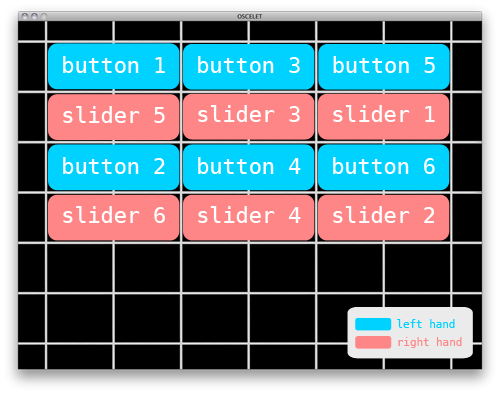
\includegraphics[width=1\textwidth]{../interfaces/1_example.png}
    \caption{First example interface prototype}
\end{figure}

\begin{figure}[p]
  \centering
    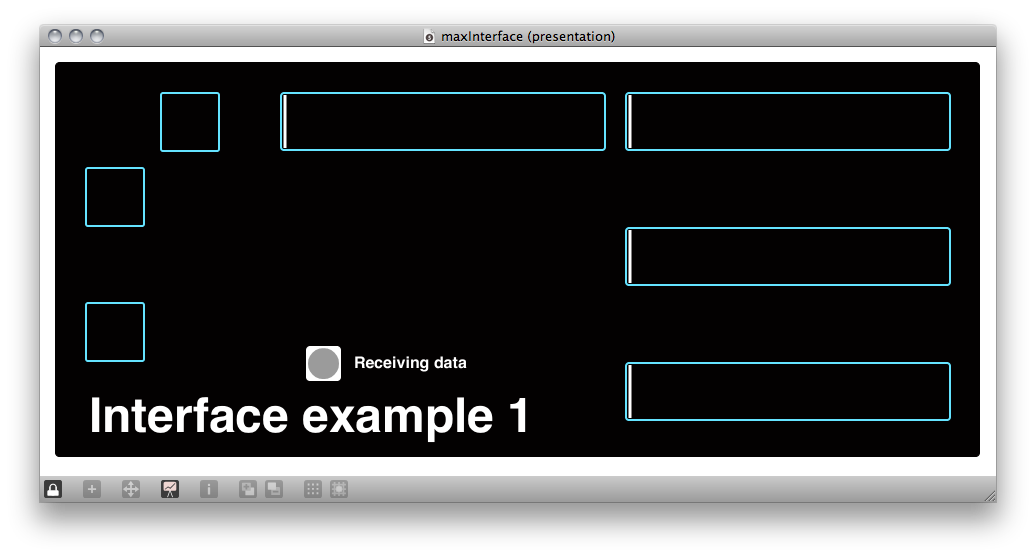
\includegraphics[width=1\textwidth]{../interfaces/1_example_max.png}
    \caption{First example interface in Max/MSP}
\end{figure}


\end{document}
